 \documentclass[final]{beamer} % beamer 3.10: do NOT use option hyperref={pdfpagelabels=false} !
  %\documentclass[final,hyperref={pdfpagelabels=false}]{beamer} % beamer 3.07: get rid of beamer warnings
  \mode<presentation> {  %% check http://www-i6.informatik.rwth-aachen.de/~dreuw/latexbeamerposter.php for examples
    \usetheme{Aalto}    %% you should define your own theme e.g. for big headlines using your own logos 
  }
  \usepackage[english]{babel}
  \usepackage[latin1]{inputenc}
  \usepackage{amsmath,amsthm, amssymb, latexsym}
  %\usepackage{times}\usefonttheme{professionalfonts}  % times is obsolete
  \usefonttheme[onlymath]{serif}
  \boldmath
  \usepackage[orientation=landscape,size=a2,scale=1.0,grid,debug]{beamerposter}                       % e.g. for DIN-A0 poster
  %\usepackage[orientation=portrait,size=a1,scale=1.4,grid,debug]{beamerposter}                  % e.g. for DIN-A1 poster, with optional grid and debug output
  %\usepackage[size=custom,width=200,height=120,scale=2,debug]{beamerposter}                     % e.g. for custom size poster
  %\usepackage[orientation=portrait,size=a0,scale=1.0,printer=rwth-glossy-uv.df]{beamerposter}   % e.g. for DIN-A0 poster with rwth-glossy-uv printer check
  % ...
  %
  \title[Morfessor Model]{Morfessor Baseline Model}
  \author[Smit et. al]{Peter Smit, Sami Virpioja, Stig-Arne Grönroos and Mikko Kurimo}
  \institute[Aalto University]{Aalto University}
  \date{April 28th, 2014}

\newlength{\columnheight}
\setlength{\columnheight}{105cm}


  \begin{document}
  \begin{frame}{Morfessor 2.0 -- Related Projects} 
\begin{columns}



\begin{column}{.49\textwidth}
  \begin{beamercolorbox}[center,wd=\textwidth]{postercolumn}
 \begin{block}{Aalto University}
              \begin{itemize}
              \item Former Helsinki University of Technology (or TKK)

		\AaltoLogoLarge{2}{''}{aaltoYellow}
              \end{itemize}              
            \end{block}
            
	\end{beamercolorbox}
\vfill
  \begin{beamercolorbox}[center,wd=\textwidth]{postercolumn}
 \begin{block}{Morpho challenge}
              \begin{itemize}
		\item Coming up: Morpho challenge 2014
              \end{itemize}              
            \end{block}
            
	\end{beamercolorbox}
\end{column}
\begin{column}{.5\textwidth}
  \begin{beamercolorbox}[center,wd=\textwidth]{postercolumn}
 \begin{block}{Simple4All}
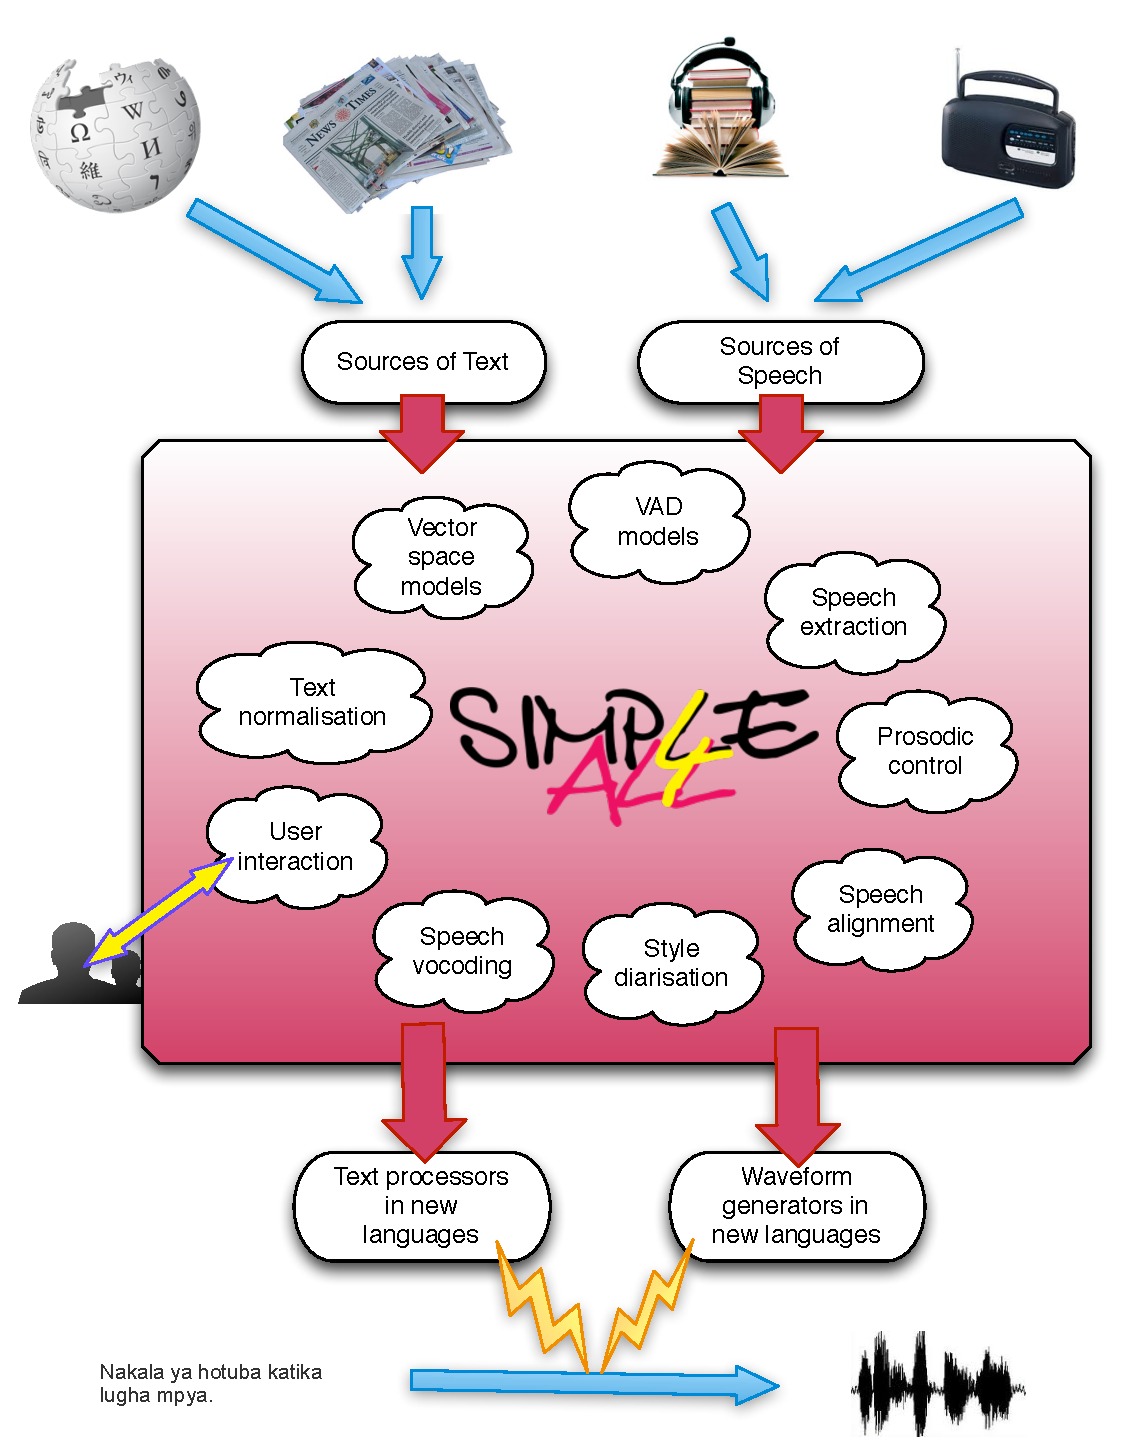
\includegraphics[width=\textwidth]{s4a}             
            \end{block}
            
	\end{beamercolorbox}
\end{column}

\end{columns}
 \end{frame}



  \end{document}
  